\documentclass[12pt]{article}

\usepackage{importantstuff}

\title{Renderização de Objetos Tridimensionais \\
\large Transformações Lineares e Espaços}

\author{Luciano Pereira Sampaio, Vitor Matheus do Nascimento}
\date{Novembro de 2023}


\begin{document}

\thispagestyle{empty}

\begin{figure}
    \centering
    
\includegraphics[width=9cm]{imgs/emap.jpg}
    \vspace{4cm}	
\end{figure}

\begin{center}
    {\huge \bf Renderização de Objetos Tridimensionais \\
    \vspace{0.5cm}
    \large Transformação Lineares e Espaços}

    \vspace{2cm}

    {Luciano Pereira Sampaio \\
    Vitor Matheus do Nascimento Moreira}
    \vfill
    Rio de Janeiro, \\
    Novembro de 2023
\end{center}
\pagebreak

\setcounter{page}{1}
\tableofcontents
\pagebreak


\section{Introdução}

No presente trabalho, iremos discutir sobre as transformações aplicadas a objetos tridimensionais de modo que eles possam ser exibidos em superficies bidimensionais, como a tela de um computador. Este é um dos assuntos de grande interesse na área da computação gráfica, e é essencial para a representação visual de objetos tridimensionais em diversos contextos, como jogos, simulações e design gráfico. A transição de um ambiente tridimensional para uma superfície bidimensional envolve uma série de transformações lineares e algoritmos que visam preservar as características essenciais dos objetos, como forma, proporção e orientação, nosso intuito é discutir tais técnicas e aplica-las para criarmos um renderizador efetivo.

\subsection{Motivação}

As aplicações do tema podem ser vistas em diversos programas importantes no dia-a-dia, desde aplicativos profissionais, como o AutoCAD e o MATLAB, aplicativos que auxiliam na visualização e construção de elementos 2D e 3D para diferentes propósitos, até contextos de entretenimento, como jogos e animações 3D.

O funcionamento desses aplicativos, incluindo o que o usuário consegue ver em sua tela, é atrelado aos conceitos de Álgebra Linear e Computação. Cada ponto e sua posição na tela deve ser uma representação gráfica coerente de um objeto de um objeto tridimensional, e para isso diversos processos são aplicados antes da visualização na tela.

Pensando nisso, acreditamos que tal assunto é de interesse tanto para a aplicação de conceitos de Álgebra Linear quanto para aplicação de conceitos de Computação, todavia, daremos ênfase para os conceitos de Álgebra Linear.

\subsection{Metodologia}

Após a definição do tema, a abordagem escolhida foi a de estudar sobre o tema e aplica-lo por meio de um renderizador programado em Python utilizando o Pygame.

Antes de prosseguirmos, existem alguns conceitos importantes para discutirmos, o primeiro é em relação a como nosso objeto tridimensional é representado. Em suma, é o melhor que podemos fazer é aproximar um objeto a partir de pontos e polígonos, entender como as transformações são aplicadas aos pontos já é o bastante para entender a representação geral do modelo. Estes pontos, com coordenadas $(x,y,z)$, são usados, usualmente, como colunas de uma matriz, e transformações lineares podem ser aplicadas a eles. Além disso, geralmente fazemos uma divisão entre três espaços de coordenadas principais, falamos sobre cada uma a seguir.

\subsection{Espaço do Mundo (World Space)}

O espaço do mundo é o espaço tridimensional no qual todos nossos objetos e nossa câmera se encontram. Sua origem é um ponto que indica o centro de nosso cenário, por convenção, consideramos o ``chão'' como o plano xz, e a altura como a componente y. 

\subsection{Espaço do Objeto (Local Space)}

O espaço do objeto é o espaço em que se encontra um objeto tridimensional individual, cada objeto diferente te seu próprio espaço. O centro do objeto é também o centro do sistema de coordenadas do espaço, 
 neste sistema representar se encontra convencionalmente centrado na sua origem, e aplicaremos transformações lineares para manipular esse objeto em relação a seu sistema de coordenadas para encontrar sua posição, orientação e tamanho no sistema de coordenadas do mundo. 


\subsection{Espaço da Câmera (View Space)}

O espaço da câmera representa o ponto de vista da nossa câmera virtual posicionada no mundo, ou seja, o espaço do mundo relativo à câmera. Existem algumas transformações envolvendo este espaço, mas acreditamos que é mais fácil explica-lás depois de explicarmos sobre projeção, então voltaremos a falar sobre a câmera. 

\section{Transformações Gerais}

Queremos que seja possível manipular cada um de nossos espaços a partir de transformações lineares, uma vez que assim poderíamos escrever uma transformação complexa a partir de uma composição de transformações mais simples. Com isso, vamos analisar e encontrar nossas principais transformações de interesse, para manipulações que mudem a orientação, posição e tamanho de um espaço.

Basicamente, queremos uma forma de rotacionar, escalar e transladar nosso objeto.
Vamos analisar cada caso:

\begin{enumerate}[noitemsep]
    \item Escala
    \item Rotação
    \item Translação
\end{enumerate}

Note que todas transformações acima podem ser realizadas representadas por matriz $3\times3$, exceto a translação, isso porque transformações lineares devem preservar a origem, mas translações não fazem isso. Entretanto, podemos contornar esse problema usando uma matriz $4\times4$, no que é conhecido como coordenadas homogêneas. Nossos vetores passam a ser do tipo $(x, y, z, w)$, e dizemos que $w = 1$.

Esse não é o único motivo pelo qual usamos coordenadas homogêneas ao lidar com renderização de objetos tridimensionais, na verdade, esse é um dos menores motivos, visto que poderíamos ``simplesmente'' somar um vetor com os fatores de translação, no entanto, utilizar um sistema de coordenadas homogêneas é essencial para outras coisas, mas não convém falar sobre isso no momento, por enquanto vamos nos contentar com a explicação da translação.

Agora, podemos encontrar transformações lineares para cada um dos três casos necessários.

\subsection{Transformação de Escala}\label{scale_transform}

Não há segredos nesta transformação, basicamente vamos multiplicar cada eixo do objeto por um escalar, vamos chamar a matriz que representa essa transformação de S.
\[
S =
\begin{bmatrix}
    S_{x} & 0 & 0 & 0 \\
    0 & S_{y} & 0 & 0 \\
    0 & 0 & S{z}  & 0 \\
    0 & 0 & 0     & 1
\end{bmatrix}
\implies
S    
\begin{bmatrix}
    x \\
    y \\
    z \\
    1
\end{bmatrix}
=
\begin{bmatrix}
    S_{x} \cdot x \\
    S_{y} \cdot y \\
    S_{z} \cdot z \\
    1
\end{bmatrix}
\]

\subsection{Transformação de Rotação/Orientação}\label{rotation_transform}

Para a rotação e orientação, vamos utilizar ângulos eulerianos. O que vamos fazer é representar rotações em torno de cada eixo dado um ângulo, já sabemos como é a rotação em duas dimensões, podemos aplicar uma rotação ``bidimensional'' considerando 2 eixos e deixando o outro eixo livre, e repetir esse processo mais duas vezes, vamos chamar as matriz que fazem essa transformação de $R_x$, $R_y$ e $R_z$.

\begin{equation}
    \begin{cases}
        y' = y \cdot \cos(\phi) - z \cdot \sin(\phi) \\
        z' = y \cdot \sin(\phi) + z \cdot \cos(\phi) \\
        x' = x
    \end{cases}
    \implies
    R_x =
    \begin{bmatrix}
        1 & 0           &           0 & 0 \\
        0 &  \cos(\phi) &  \sin(\phi) & 0 \\ 
        0 & -\sin(\phi) &  \cos(\phi) & 0 \\
        0 & 0           &           0 & 1 
    \end{bmatrix}    
\end{equation}


\begin{equation}
    \begin{cases}
        z' = z \cdot \cos(\theta) - x \cdot \sin(\theta) \\
        x' = z \cdot \sin(\theta) + x \cdot \cos(\theta) \\
        y' = y
    \end{cases} 
    \implies
    R_y =
    \begin{bmatrix}
        \cos(\theta)  & 0 &  \sin(\theta) & 0 \\ 
        0             & 1 &            0  & 0 \\
        -\sin(\theta) & 0 &  \cos(\theta) & 0 \\
        0             & 0 &            0  & 1 
    \end{bmatrix}
\end{equation}


\begin{equation}
    \begin{cases}
        x' = x \cdot \cos(\psi) - y \cdot \sin(\psi) \\
        y' = x \cdot \sin(\psi) + y \cdot \cos(\psi) \\
        z' = z 
    \end{cases}
    \implies
    R_z =
    \begin{bmatrix}
        \cos(\psi) & -\sin(\psi) & 0 & 0 \\ 
        \sin(\psi) &  \cos(\psi) & 0 & 0 \\
        0          &           0 & 1 & 0 \\
        0          &           0 & 0 & 1 
    \end{bmatrix}
\end{equation}

A partir disso, podemos demonstrar a orientação de qualquer objeto tridimensional dado seus ângulos em relação a cada eixo. É muito importante notar que essas matrizes não comutam, então a ordem das transformações importa, e precisamos pensar nelas na hora de escolher os ângulos para orientação. Além disso, a composição dessas matrizes para representar uma rotações pode levar a um problema conhecido como ``Gimbal Lock'', no qual se perde um grau de liberdade da rotação, mas resolver esse problema foge do escopo, e ângulos eulerianos funcionam perfeitamente para representar uma orientação.

\subsection{Transformação de Translação}\label{translation_transform}

Por fim, outra transformação que precisamos é a de translação, como falamos anteriormente, aqui nos é conveniente utilizar coordenadas homogêneas para que a translação possa ser representada como uma transformação linear. Em coordenadas homogêneas, uma transformação de cisalhamento, é capaz de somar vetores à nossos vetores originais. Chamamos a matriz dessa transformação de $T$.

\[
T =
\begin{bmatrix}
    1 & 0 & 0 & T_{x} \\
    0 & 1 & 0 & T_{y} \\
    0 & 0 & 1 & T_{z} \\
    0 & 0 & 0 & 1 \\
\end{bmatrix}
\implies
\begin{bmatrix}
    1 & 0 & 0 & T_{x} \\
    0 & 1 & 0 & T_{y} \\
    0 & 0 & 1 & T_{z} \\
    0 & 0 & 0 & 1 \\
\end{bmatrix}
\begin{bmatrix}
    x \\
    y \\
    z \\
    1
\end{bmatrix} 
=
\begin{bmatrix}
    x + T_{x}\\
    y + T_{y}\\
    z + T_{z}\\
    1
\end{bmatrix}
\]

Perceba que acabamos de representar o deslocamento de um vetor através de uma transformação linear, então acabamos de encontrar todas transformações necessárias para manipular a posição, orientação  e tamanho de um objeto tridimensional.


\section{Objetos}

Aqui, queremos representar nossos objetos nas coordenadas do Espaço do Mundo, o que fazemos, para isso aplicamos as transformações lineares que encontramos nos tópicos anteriores, a fim de demonstrar o tamanho, orientação e posição dos objetos no mundo.

Nossas transformações são as seguintes:

\subsection{Escala no Objeto}

Aplicamos a matriz de escala encontrada na subseção {\ref{scale_transform}} a fim de mudarmos a altura, largura e comprimento do nosso objeto. Como mostrado na figura abaixo:

\begin{figure}[H]
    \centering
    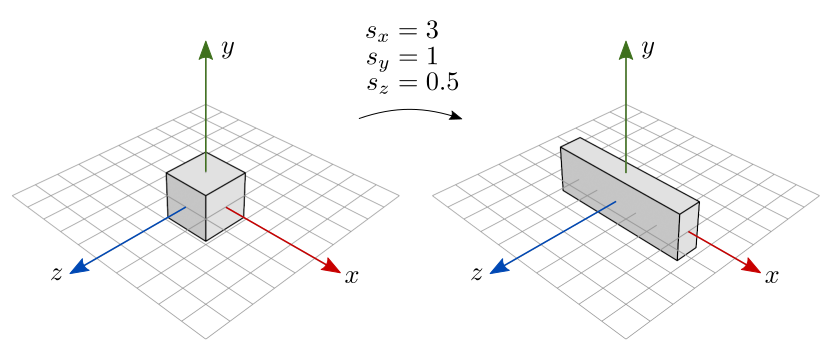
\includegraphics[width=0.6\linewidth]{imgs/07_scaling4.png}
    \caption{Exemplo de escala em um objeto}
\end{figure}

\subsection{Rotacionando o Objeto}

Aqui fazemos uma composição entre as matrizes de rotação dos eixos encontradas na subseção {\ref{rotation_transform}}. Por exemplo, $R_x R_y R_z$. É importante notar que as matriz de rotações não comutam em $\mathbb{R}^3$, e os ângulos devem ser escolhidos pensando nisso.

\begin{figure}[H]
    \centering
    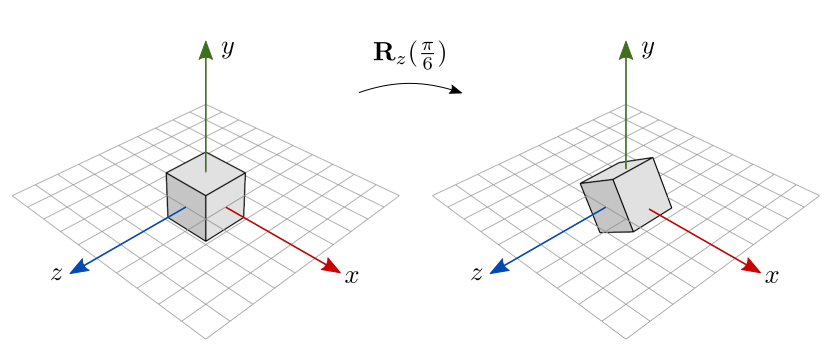
\includegraphics[width=0.6\linewidth]{imgs/07_rotation5.png}
    \caption{Exemplo de rotação em um objeto}
\end{figure}

\subsection{Transladando o Objeto}

Por fim, aplicamos a translação no objeto dada a matriz encontrada na subseção {\ref{translation_transform}}, conforme a posição do objeto em relação ao Espaço do Mundo.

\begin{figure}[H]
    \centering
    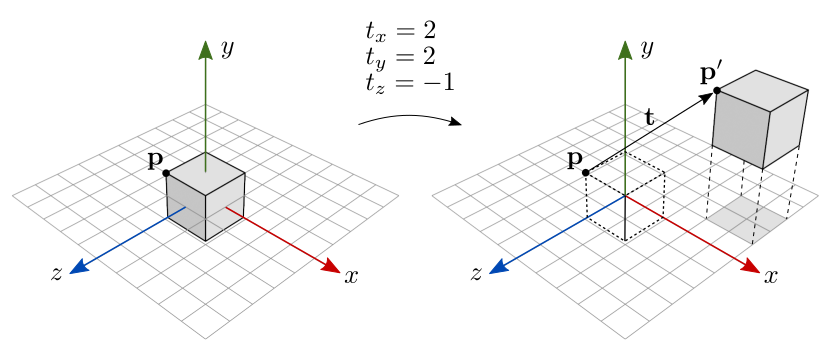
\includegraphics[width=0.6\linewidth]{imgs/07_translation1.png}
    \caption{Exemplo de translação em um objeto}
\end{figure}

\noindent
Com isso, a matriz final que leva o objeto para o espaço do mundo é:
\\[\baselineskip]
\boldmath{}
$M_{obj} = T \cdot R_x \cdot R_y \cdot R_z \cdot S$
\unboldmath{}

\section{Câmera}

Aqui iremos falar sobre a câmera. Dois pontos importantes sobre a câmera, são que queremos que ela possa ``apontar'' para qualquer local do espaço do mundo, e queremos que ela pode estar localizada em qualquer local no espaço do mundo. Além disso, queremos conseguir as coordenadas dos objetos em relação à câmera, faremos isso a seguir.

\subsection{Orientação da Câmera}

Assim como os objetos, a câmera também possui uma orientação relativa ao Espaço do Mundo. 

Vamos construir a orientação da câmera com base em um sistema conhecido como ``LookAt''. Esse sistema consiste em definir um vetor que indica a direção para onde a câmera aponta, e criar uma base ortonormal a partir desse vetor.

\subsubsection{Câmera LookAt}

\boldmath{}
Queremos encontrar uma base ortonormal \boldmath{$\{u,v,n\}$} para o espaço da câmera, considerando que temos as seguintes informações:

\begin{enumerate}[noitemsep]
    \item Um ponto $P_{cam}$ no Espaço do Mundo, relativo à posição da câmera.
    \item Um ponto arbitrário $P_{at}$ no Espaço do Mundo, relativo a posição que a câmera aponta.
    \item Um vetor $V_{up}$, que indica a direção ``para cima'', geralmente  o vetor $\begin{bmatrix}
        0 & 1 & 0
    \end{bmatrix}^T$. 
\end{enumerate}

\begin{figure}[H]
    \centering
    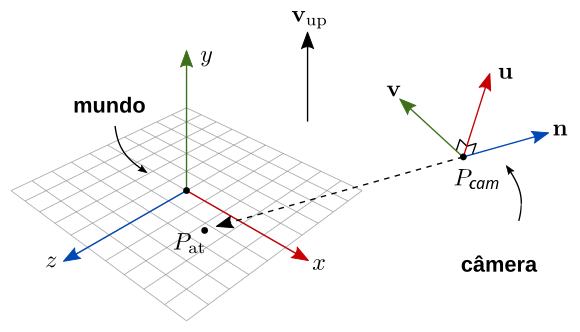
\includegraphics[width=0.6\linewidth]{imgs/07_lookat1.png}
    \caption{Representação dos Espaços do Mundo e Câmera}
\end{figure}

\noindent
Perceba que o vetor $n$ pode ser encontrado da seguinte forma: $n =\frac{P_{cam}-P_{at}}{|P_{cam}-P_{at}|}$.
Ora, então o vetor $u$ é dado por: $u =\frac{v_{up} \times n}{|v_{up} \times n|}$. E de forma parecida: $v = u \times n$. Como $n$ e $u$ já são vetores normalizados e ortogonais, seu produto cruzado já está normalizado.
\\~\\
Com isso, a matriz que define a orientação da câmera no espaço do mundo é:

\unboldmath{}

\[
R_{cam} =
\begin{bmatrix}
    u_1 & v_1 & n_1 & 0   \\
    u_2 & v_2 & n_2 & 0   \\    
    u_3 & v_3 & n_3 & 0   \\
    0 & 0 & 0 & 1
\end{bmatrix}
\]

\noindent
Onde, os indices 1, 2 e 3 correspondem à respectiva entrada do vetor.
    
\subsection{Posição da Câmera}

Perceba que a matriz que encontramos acima nos dá a orientação da câmera em relação ao Mundo, mas ainda precisamos posicionar a câmera no Espaço do Mundo. A matriz que usamos aqui é a mesma que usamos para posicionar os Objetos.

\[
T_{cam} =
\begin{bmatrix}
    1 & 0 & 0 & T_{x} \\
    0 & 1 & 0 & T_{y} \\
    0 & 0 & 1 & T_{z} \\
    0 & 0 & 0 & 1 \\
\end{bmatrix}
\]

\subsection{Transformação Final da Câmera}

Compondo as transformações que encontramos acima temos o seguinte:

\[
M_{cam} = T_{cam} R_{cam} = 
\begin{bmatrix}
    1 & 0 & 0 & T_{x} \\
    0 & 1 & 0 & T_{y} \\
    0 & 0 & 1 & T_{z} \\
    0 & 0 & 0 & 1 \\
\end{bmatrix}
\begin{bmatrix}
    u_1 & v_1 & n_1 & 0   \\
    u_2 & v_2 & n_2 & 0   \\    
    u_3 & v_3 & n_3 & 0   \\
    0 & 0 & 0 & 1
\end{bmatrix}
\]

\noindent
Isso nos dá a posição e orientação da câmera nas coordenadas do mundo, como mostrado na figura abaixo.

\begin{figure}[H]
    \centering
    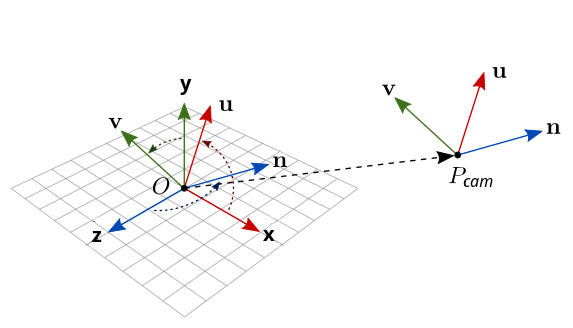
\includegraphics[width=0.6\linewidth]{imgs/07_lookat7.png}
    \caption{Mudança do espaço da câmera para o espaço do mundo}
\end{figure}

\section{Espaço do Mundo para Espaço da Câmera}

No momento, temas a posição e orientação dos objetos em relação ao mundo, temos também a posição e orientação da câmera no mundo. O que gostaríamos é conseguir as coordenadas dos objetos da cena em relação à câmera.

\begin{figure}[H]
    \centering
    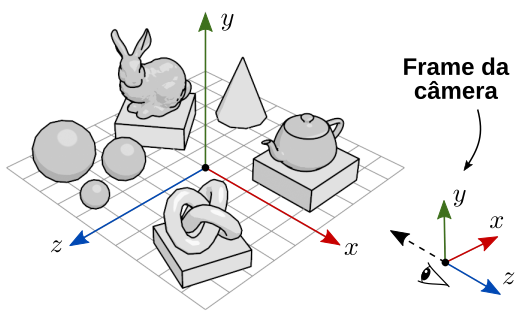
\includegraphics[width=0.6\linewidth]{imgs/07_glspace7.png}
    \caption{Espaço da câmera em relação ao espaço do mundo}
\end{figure}

Como queremos as coordenadas dos objetos em relação à câmera, precisamos fazer uma mudança de base do Espaço do Mundo para o nosso Espaço da Câmera. Felizmente, a matriz que encontramos para posicionar e orientar a câmera é facilmente invertível.

Como vimos anteriormente, a matriz que posiciona nossa câmera no mundo é dada por:
\[
M_{cam} = T_{cam} R_{cam} = 
\begin{bmatrix}
    1 & 0 & 0 & T_{x} \\
    0 & 1 & 0 & T_{y} \\
    0 & 0 & 1 & T_{z} \\
    0 & 0 & 0 & 1 \\
\end{bmatrix}
\begin{bmatrix}
    u_1 & v_1 & n_1 & 0   \\
    u_2 & v_2 & n_2 & 0   \\    
    u_3 & v_3 & n_3 & 0   \\
    0 & 0 & 0 & 1
\end{bmatrix}
\]

Uma vez que $R_{cam}$ nada mais é que uma matriz de rotação, sua inversa é igual a sua transposta. Portanto, temos o seguinte:

\[
M_{cam}^{-1} = R_{cam}^T T_{cam}^{-1} = 
\begin{bmatrix}
    u_1 & u_2 & u_3 & 0   \\
    v_1 & v_2 & v_3 & 0   \\    
    n_1 & n_2 & n_3 & 0   \\
    0 & 0 & 0 & 1
\end{bmatrix}
\begin{bmatrix}
    1 & 0 & 0 & -T_{x} \\
    0 & 1 & 0 & -T_{y} \\
    0 & 0 & 1 & -T_{z} \\
    0 & 0 & 0 & 1 \\
\end{bmatrix}
\]

\section{Projeção}

Agora que já orientamos e posicionamos os objetos em nossa cena e agora que já temos as coordenadas dos objetos relativas à câmera, podemos começar a pensar sobre como exibir efetivamente nossos objetos na tela do computador, ou seja, pensar em como projetar nosso espaço tridimensional em um espaço bidimensional. Existem algumas formas de fazer isso, em principal existe a projeção ortográfica e a projeção perspectiva, focaremos na projeção perspectiva, uma vez que essa preserva a noção de profundidade. 


\subsection{Projeção perspectiva}

Neste tipo de projeção, queremos que quanto mais distantes do centro de visão os objetos estejam, menores eles fiquem quando projetados. Nossa projeção perspectiva será responsável por: ajustar as coordenadas x e y com base no tamanho da tela (corrigir o aspect ration), ajustar as coordenadas x e y com base no ângulo de visão que definirmos, e normalizar os valores de x, y e z para que eles fiquem entre -1 e 1, tal normalização é chamada de NDC (Normalized Device Coordinates). 

\begin{figure}[H]
    \centering
    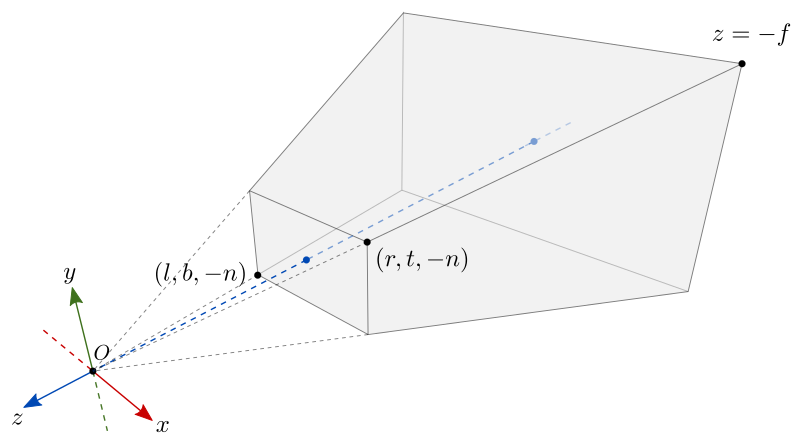
\includegraphics[width=0.6\linewidth]{imgs/08_projection7.png}
    \caption{Volume de visão para a projeção perspectiva}
\end{figure}

Os parâmetros que definem nossa pirâmide truncada são l (left), r (right), b (bottom), t (top), n (near) e f (far), sendo que l, r, b e t indicam as coordenadas da tela em relação a uma origem arbitrária (esses parâmetros normalmente estão em unidade de pixels), e n e f definem os planos de corte da visão (visão minima e máxima).

\subsubsection{Contrução da Matriz de perspectiva}

Para facilitar os cálculos, consideramos que o centro da projeção coincide com a origem do mundo, e o que o eixo onde a câmera alinhado com o eixo z do mundo.
Agora, definindo dois planos normais ao eixo $Z$, o mais próximo da origem representando a tela do computador e com posição $Z = -n$, e o mais distante representando o plano máximo de visão (até onde enxergamos), com $Z = -f$.

\begin{figure}[H]
    \centering
    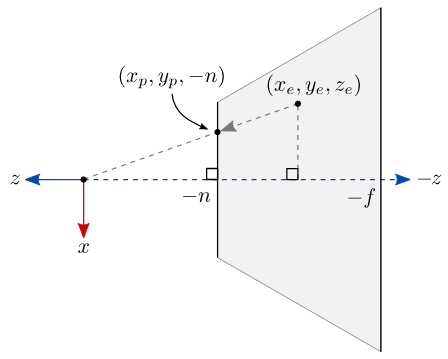
\includegraphics[width=0.6\linewidth]{imgs/projection02.png}
    \caption{Volume de visão visto de cima}
\end{figure} 


Após projeção do ponto $(X_e,Y_e,Z_e)$ o mesmo passa a ter coordenadas $(X_p, Y_p, -n)$. Através da razão de triângulos semelhantes temos:

\[
\frac{X_p}{-n} = \frac{X_e}{Z_e} \implies X_p = \frac{n \cdot X_e}{-Z_e}
\]

O mesmo vale para $Y_p$:

\[
\frac{Y_p}{-n} = \frac{Y_e}{Z_e} \implies Y_p = \frac{n \cdot Y_e}{-Z_e}
\]

Perceba que precisamos fazer uma divisão por $-Z_e$ para encontrar as coordenadas de $X_p$ e $Y_p$, o problema é não existe transformação linear que faça isso neste caso. Mas como estamos trabalhando com coordenadas homogêneas, podemos usar um pequeno truque:

\[
\begin{bmatrix}
    x_c \\
    y_c \\
    z_c \\
    w_c
\end{bmatrix}
=
\begin{bmatrix}
    . & . & . & . \\
    . & . & . & . \\
    . & . & . & . \\
    0 & 0 & -1 & 0
\end{bmatrix}
\begin{bmatrix}
    x_e \\
    y_e \\
    z_e \\
    1
\end{bmatrix}
=
\begin{bmatrix}
    x_c \\
    y_c \\
    z_c \\
    -z_e
\end{bmatrix}
\]

Como quereremos normalizar nosso volume de visão em um cubo, temos o seguinte a seguinte mapeamento entre os intervalos:

\begin{itemize}
    \item Em x: [l,r], no espaço da câmera, para [-1,1] em NDC
    \item Em y: [b,t], no espaço da câmera, para [-1,1] em NDC
    \item Em z: [-n,-f], no espaço da câmera, para [-1,1] em NDC
\end{itemize}

\begin{figure}
    \centering
    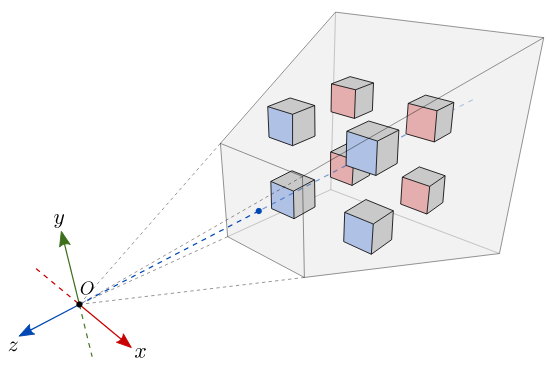
\includegraphics[height=0.3\linewidth]{imgs/Screenshot 2023-11-20 at 15-40-45 8.2 Projeção perspectiva MCTA008-17 Computação Gráfica.png}
    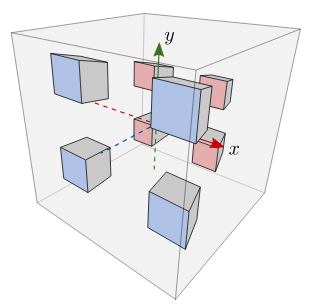
\includegraphics[height=0.3\linewidth]{imgs/Screenshot 2023-11-20 at 22-31-11 8.2 Projeção perspectiva MCTA008-17 Computação Gráfica.png}
    \caption{Objetos dentro do volume de visão antes e após a normalização.}
\end{figure}

\noindent
Com isso

\[
    x_{ndc} = a_x x_p + b_x
\]
\[    
    y_{ndc} = a_y y_p + b_y
\]

\noindent
Onde a e b são respectivamente fatores de escala e translação.

\[
    a_x = \frac{2}{r-l}, \qquad b_x = -\frac{r+l}{r-l}
\]
\[
    a_y = \frac{2}{t-b}, \qquad b_y = -\frac{t+b}{t-b}
\]

\noindent
Isso nos dá

\[
    x_c = n \cdot a_x \cdot x_e - b_x \cdot z_e
\]
\[
    y_c = n \cdot a_y \cdot y_e - b_y \cdot z_e
\]

Mudando os elementos da matriz de projeção:

\[
\begin{bmatrix}
    x_c \\
    y_c \\
    z_c \\
    w_c
\end{bmatrix}
=
\begin{bmatrix}
    \frac{2n}{r-l} & 0 & \frac{r+l}{r-l} & 0 \\
    0 & \frac{2n}{r-l} & \frac{t+b}{t-b} & 0 \\
    0 & 0 & \alpha & \beta \\
    0 & 0 & -1 & 0
\end{bmatrix}
\begin{bmatrix}
    x_e \\
    y_e \\
    z_e \\
    1
\end{bmatrix}    
\]

Sabendo que precisamos mapear o intervalo [-n, -f] para [-1,1], podemos forma um sistema de equações:

\[
\begin{cases}
    \frac{-\alpha \cdot n + \beta}{n} = -1 \\
    \frac{-\alpha \cdot f + \beta}{f} = 1
\end{cases}
\implies
-\alpha n + \beta = -n, \quad  -\alpha f + \beta = -f
\]

\noindent
Com isso:

\[
\begin{cases}
    \alpha = -\frac{f+n}{f-n} \\
    \beta = -\frac{2fn}{f-n}
\end{cases}    
\]

\noindent
Com isso, nossa matriz de perspectiva é:

\[
M_{persp} =
\begin{bmatrix}
    \frac{2n}{r-l} & 0 & \frac{r+l}{r-l} & 0 \\    
    0 & \frac{2n}{t-b} & \frac{t+b}{t-b} & 0 \\    
    0 & 0 & -\frac{f+n}{f-n} & -\frac{2fn}{f-n} \\
    0 & 0 & -1 & 0 
\end{bmatrix}    
\]

\begin{figure}[H]
    \centering
    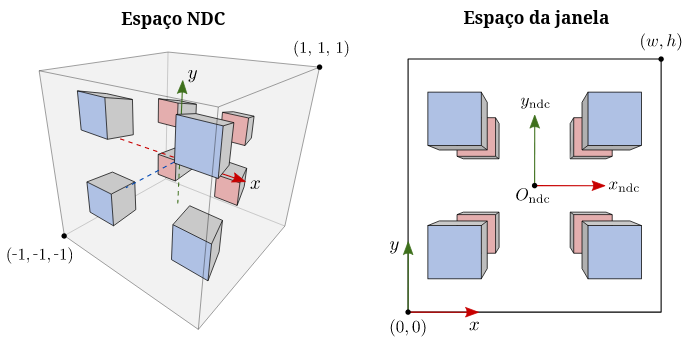
\includegraphics[height=0.4\linewidth]{imgs/Screenshot 2023-11-20 at 22-32-44 8.2 Projeção perspectiva MCTA008-17 Computação Gráfica.png}
    \caption{Objetos em NDC e correspondentes no espaço da tela.}
\end{figure}

\noindent
Se o centro da nossa tela for a origem para a perspectiva, então $r = -l$ e $t = -b$, e a matriz é simplificada para:

\[
M_{persp} =
\begin{bmatrix}
    \frac{n}{r} & 0 & 0 & 0 \\    
    0 & \frac{n}{t} & 0 & 0 \\    
    0 & 0 & -\frac{f+n}{f-n} & -\frac{2fn}{f-n} \\
    0 & 0 & -1 & 0 
\end{bmatrix}    
\]


Podemos também utilizar o ângulo de visão para definir a matriz, chamamos de $\theta$ a abertura do campo de visão (FOV). Chamamos de razão de espectro a = $\frac{width}{height}$, onde ``width'' é o comprimento da tela e ``height'' é a altura da tela, e n e f são os planos de recorte próximo  (near) e distante (far).
\\~\\
Então:

\[
\frac{t}{n} = \tan(\frac{\theta}{2})    
\]
\[
t = n\tan(\frac{\theta}{2})    
\]

E por simetria b = -t

\begin{figure}[H]
    \centering
    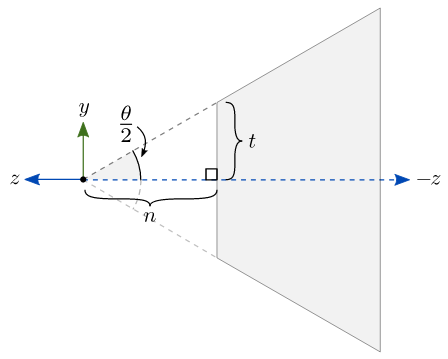
\includegraphics[width=0.6\linewidth]{imgs/Screenshot 2023-11-20 at 18-58-22 8.2 Projeção perspectiva MCTA008-17 Computação Gráfica.png}
    \caption{Ângulo de abertura do campo de visão vertical. }
\end{figure}

\[
r=t\frac{w}{h} = t \cdot a    
\implies
M_{persp} =
\begin{bmatrix}
    \frac{1}{a \cdot \tan(\frac{\theta}{2})} & 0 & 0 & 0 \\    
    0 & \frac{1}{\tan(\frac{\theta}{2})} & 0 & 0 \\    
    0 & 0 & -\frac{f+n}{f-n} & -\frac{2fn}{f-n} \\
    0 & 0 & -1 & 0 
\end{bmatrix}    
\]

\noindent
No entanto, nossas coordenadas x e y agora se encontram no intervalo [-1,1], precisamos transformar esse intervalo no intervalo respectivo da nossa tela, ou seja, precisamos multiplicar as coordenadas x e y por metade da largura e metade altura da tela, respectivamente. Isso é feito facilmente com a matriz a seguir:

\[
M_{vport} =
\begin{bmatrix}
    \frac{w}{2} & 0 & 0 & 0 \\
    0 & \frac{h}{2} & 0 & 0 \\
    0 & 0 & 1 & 0 \\
    0 & 0 & 0 & 1
\end{bmatrix}    
\]

\section{Compondo as Transformações}

Agora já temos todas transformações necessárias para rotacionar, escalar e posicionar qualquer objeto tridimensional em nossa cena, bem como escolher uma posição e orientação para nossa câmera, além de termos implementado uma projeção perspectiva para visualização mais fiel à realidade. Vamos ver agora como a composição das matrizes se parece agora.
\\~\\
Recapitulando, primeiros encontramos as coordenadas dos objetos no mundo, aplicando as seguintes transformações:

\boldmath{}
\[
M_{obj} = T \cdot R \cdot S
\]
\unboldmath{}

\noindent
Onde:
\\[\baselineskip]
$T = 
\begin{bmatrix}
    1 & 0 & 0 & T_{x} \\
    0 & 1 & 0 & T_{y} \\
    0 & 0 & 1 & T_{z} \\
    0 & 0 & 0 & 1 \\
\end{bmatrix}$
\\[\baselineskip]
$R =
\begin{bmatrix}
    \cos(\psi) & -\sin(\psi) & 0 & 0 \\ 
    \sin(\psi) &  \cos(\psi) & 0 & 0 \\
    0          &           0 & 1 & 0 \\
    0          &           0 & 0 & 1 
\end{bmatrix}
\begin{bmatrix}
    \cos(\theta)  & 0 &  \sin(\theta) & 0 \\ 
    0             & 1 &            0  & 0 \\
    -\sin(\theta) & 0 &  \cos(\theta) & 0 \\
    0             & 0 &            0  & 1 
\end{bmatrix}
\begin{bmatrix}
    1 & 0           &           0 & 0 \\
    0 &  \cos(\phi) &  \sin(\phi) & 0 \\ 
    0 & -\sin(\phi) &  \cos(\phi) & 0 \\
    0 & 0           &           0 & 1 
\end{bmatrix}
$
\\[\baselineskip]
$ S =
\begin{bmatrix}
    S_{x} & 0 & 0 & 0 \\
    0 & S_{y} & 0 & 0 \\
    0 & 0 & S{z}  & 0 \\
    0 & 0 & 0     & 1
\end{bmatrix}
$
\\[\baselineskip]
A transformação que nos leva das coordenadas relativas ao mundo para as coordenadas relativas à câmera é dada por:

\boldmath{}
\[
M_{cam}^{-1} = R_{cam}^T T_{cam}^{-1}
\]
\unboldmath{}

\noindent
Onde:
\\[\baselineskip]
$R_{cam}^T =
\begin{bmatrix}
    u_1 & u_2 & u_3 & 0   \\
    v_1 & v_2 & v_3 & 0   \\    
    n_1 & n_2 & n_3 & 0   \\
    0 & 0 & 0 & 1
\end{bmatrix}
$
\\[\baselineskip]
$T_{cam}^{-1} = 
\begin{bmatrix}
    1 & 0 & 0 & -T_{x} \\
    0 & 1 & 0 & -T_{y} \\
    0 & 0 & 1 & -T_{z} \\
    0 & 0 & 0 & 1 \\
\end{bmatrix}
$
\\[\baselineskip]
A transformação que cria a perspectiva e a ajusta o  tamanho da tela é dada por:

\boldmath{}
\[
M_{view} = M_{vport} \cdot M_{persp}    
\]
\unboldmath{}

\noindent
Onde:
\\[\baselineskip]
$M_{vport} =
\begin{bmatrix}
    \frac{w}{2} & 0 & 0 & 0 \\
    0 & \frac{h}{2} & 0 & 0 \\
    0 & 0 & 1 & 0 \\
    0 & 0 & 0 & 1
\end{bmatrix}   $ 
\\[\baselineskip]
$M_{persp} =
\begin{bmatrix}
    \frac{1}{a \cdot \tan(\frac{\theta}{2})} & 0 & 0 & 0 \\    
    0 & \frac{1}{\tan(\frac{\theta}{2})} & 0 & 0 \\    
    0 & 0 & -\frac{f+n}{f-n} & -\frac{2fn}{f-n} \\
    0 & 0 & -1 & 0 
\end{bmatrix}$
\\[\baselineskip]
Nosso vetores agora são dados por:
\noindent
\boldmath{}
$
\begin{bmatrix}
x_{view} \\
y_{view} \\
z_{view} \\
w_{view}
\end{bmatrix}
=
M_{view} \cdot M_{cam}^{-1} \cdot M_{obj} \cdot 
\begin{bmatrix}
x_{obj} \\
y_{obj} \\
z_{obj} \\
1    
\end{bmatrix}
$
\unboldmath{}
\\[\baselineskip]
E por fim, para obter a posição X e Y no espaço da tela, fazemos a transformação não linear de dividir por W (perspective divide):
\\[\baselineskip]
$
\begin{bmatrix}
x_{screen} \\
y_{screen} \\
z' \\
1
\end{bmatrix}
=
\frac{1}{w_{view}}
\begin{bmatrix}
    x_{view} \\
    y_{view} \\
    z_{view} \\
    w_{view}
\end{bmatrix}
$
\\[\baselineskip]
Agora estamos prontos para exibir os nossos objetos tridimensionais na tela a partir das coordenadas $x_{screen}$ e $y_{screen}$, a coordenada $z'$ embora não seja utilizada neste trabalho, é importante para ordenar os polígonos de nossos objetos, por isso fizemos a projeção pensando em manter essa características da ordenação.


\phantomsection
\begin{thebibliography}{9}

    \bibitem{Lengyel2003}
    Eric Lengyel,
    \textit{Mathematics for 3D Game Programming and Computer Graphics},
    2nd edition,
    Cengage Learning, 2003.

    \bibitem{MCTA008-17}
        Bruno Dorta,
        \textit{Computação Gráfica},
        2017,
        \url{https://www.brunodorta.com.br/cg/},
        Accessed Nov. 2023.

    \bibitem{3DGraphicsPlaylist}
        YouTube,
        \textit{3D Graphics Playlist},
        \url{https://www.youtube.com/playlist?list=PLYnrabpSIM-97qGEeOWnxZBqvR_zwjWoo},
        Accessed Nov. 2023.
    
\end{thebibliography}


\end{document}


